\documentclass{beamer}

\usetheme{default}

\usepackage{times}

\logo{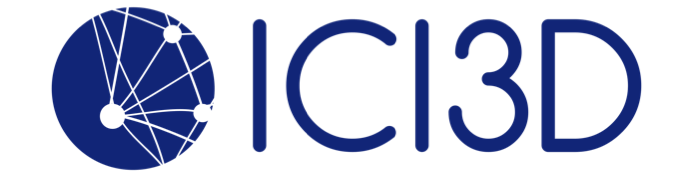
\includegraphics[width=1in]{ICI3D_logo.png}}
\setbeamertemplate{footline}[frame number]
\setbeamertemplate{navigation symbols}{}

\makeatletter
\setbeamertemplate{sidebar canvas right}{}
\setbeamertemplate{sidebar right}{%
	%\hspace{-35ex}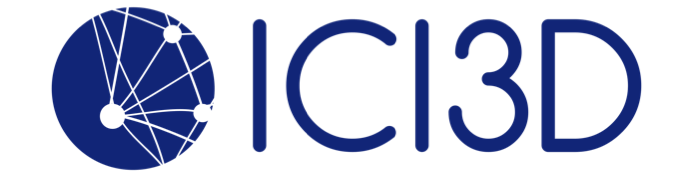
\includegraphics[width=3.5cm]{ICI3D_logo.png}
	\llap{\insertlogo\hskip0.1cm}%
	\vspace*{\fill}
}
\makeatother



\usepackage{xpatch}
\xpatchcmd{\itemize}
{\def\makelabel}
	{\ifnum\@itemdepth=1\relax
		\setlength\itemsep{2ex plus 3ex minus 2ex}% separation for first level
	\else
	\ifnum\@itemdepth=2\relax
		\setlength\itemsep{1ex plus 2ex minus 1ex}% separation for second level
	\else
	\ifnum\@itemdepth=3\relax
		\setlength\itemsep{0.5ex plus 1ex minus 0.5ex}% separation for third level
\fi\fi\fi\def\makelabel
}{}{}



\usepackage{graphicx,xspace}
\usepackage{grffile}
\usepackage{hyperref}
\usepackage{url}

\begin{document}
\begin{frame}

\frametitle{How do we use statistics}\begin{itemize}

\item We use statistics to confirm effects, estimate parameters, and
	predict outcomes

\item It usually rains when I'm in Cape Town, but mostly on Sunday\begin{itemize}

\item \emph{Confirmation:} In Cape Town, it rains more on Sundays than
		other days

\item \emph{Estimation:} In Cape Town, the \emph{odds} of rain on
		Sunday are 1.6--2.2 times higher than on other days

\item \emph{Prediction:} I am confident that it will rain at least one
		Sunday the next time I go\end{itemize}\end{itemize}
\end{frame}

\begin{frame}


\frametitle{Raining in Cape Town}

\begin{columns}[c] \column{0.54\textwidth} \small\begin{itemize}

\item How we interpret data like this necessarily depends on assumptions:\begin{itemize}

\item Is it likely our observations occured by chance?

\item Is it likely they \emph{didn't}?\end{itemize}\end{itemize}

\column{0.4\textwidth}

\hfill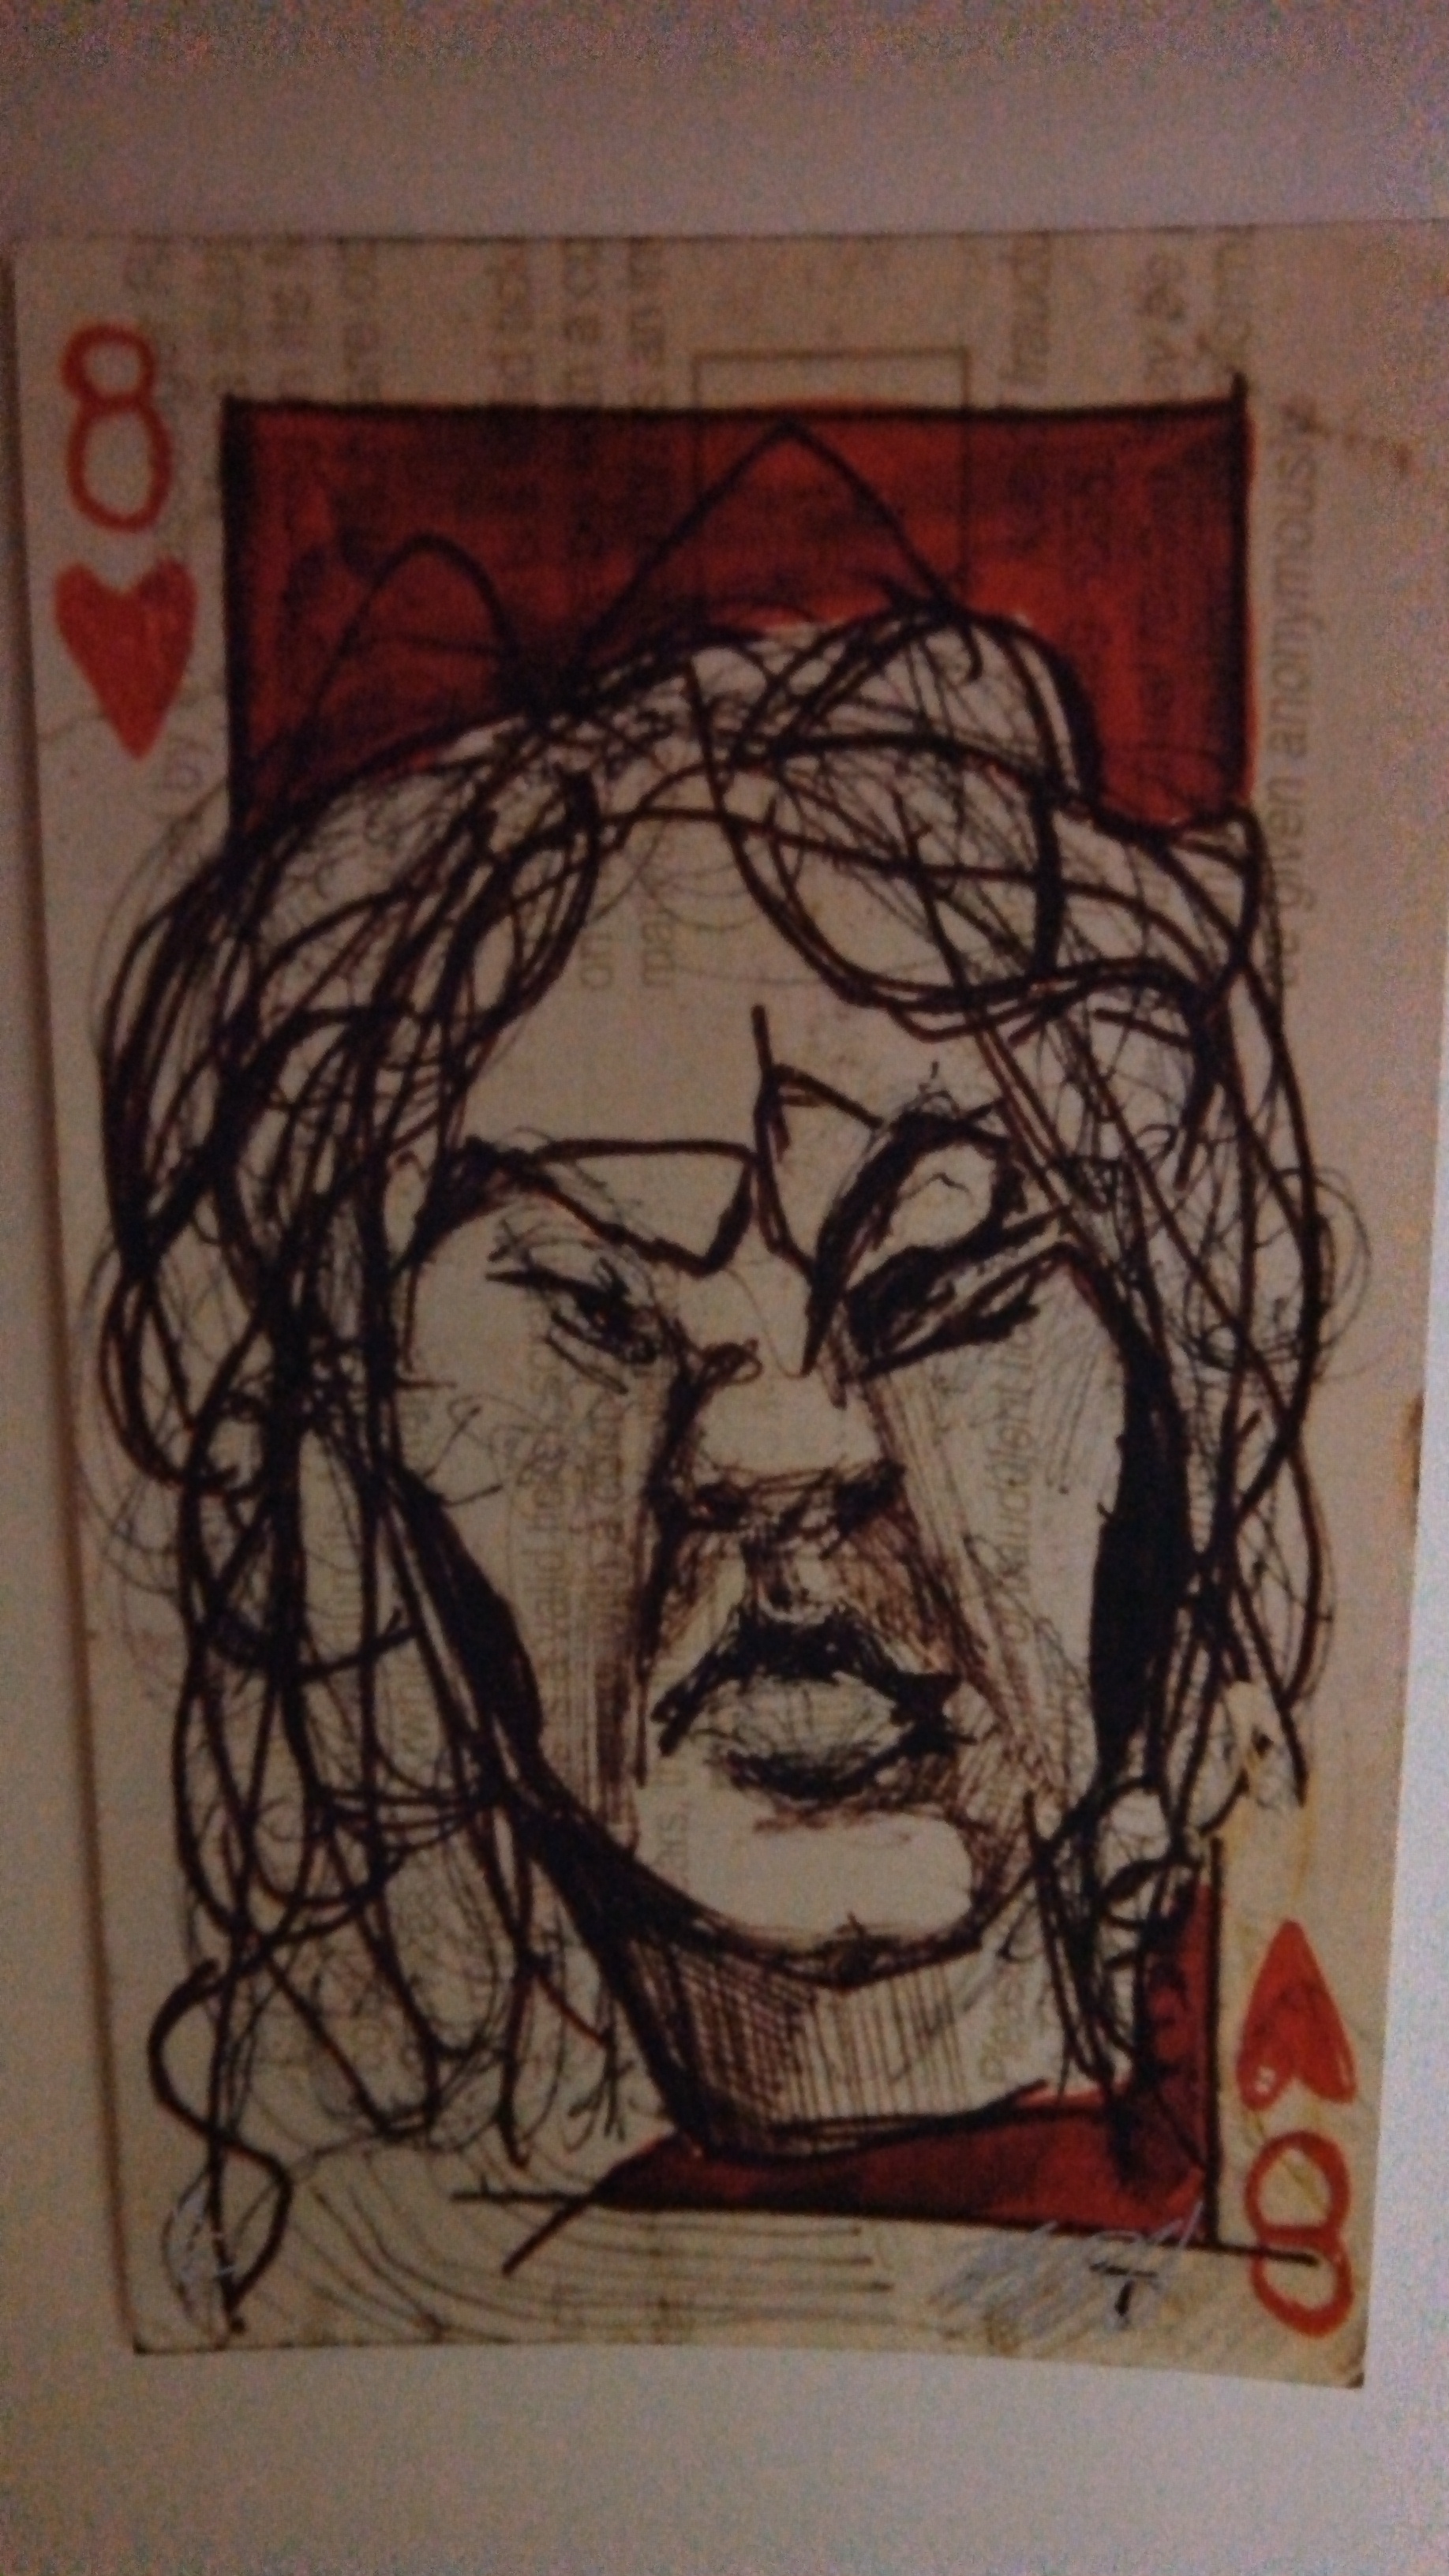
\includegraphics[height=0.8\textheight]{eight.jpg}\hfill\mbox{}

{\small\emph{Tessa Wessels, {\em Faces on a Train}}}

\end{columns}
\end{frame}

\end{document}
